%%%%%%%%%%%%%%%%%%%%%%%%%%%%%%%%%%%%%%%%%
% baposter Landscape Poster
% LaTeX Template
% Version 1.0 (11/06/13)
%
% baposter Class Created by:
% Brian Amberg (baposter@brian-amberg.de)
%
% This template has been downloaded from:
% http://www.LaTeXTemplates.com
%
% License:
% CC BY-NC-SA 3.0 (http://creativecommons.org/licenses/by-nc-sa/3.0/)
%
%%%%%%%%%%%%%%%%%%%%%%%%%%%%%%%%%%%%%%%%%

%----------------------------------------------------------------------------------------
%	PACKAGES AND OTHER DOCUMENT CONFIGURATIONS
%----------------------------------------------------------------------------------------

\documentclass[landscape,a0paper,fontscale=0.285]{baposter} % Adjust the font scale/size here

\usepackage{graphicx} % Required for including images
\graphicspath{{figures/}} % Directory in which figures are stored

\usepackage{amsmath} % For typesetting math
\usepackage{amssymb} % Adds new symbols to be used in math mode
\usepackage{wrapfig}

\usepackage{capt-of}

\usepackage{booktabs} % Top and bottom rules for tables
\usepackage{enumitem} % Used to reduce itemize/enumerate spacing
\usepackage{palatino} % Use the Palatino font
\usepackage[font=small,labelfont=bf]{caption} % Required for specifying captions to tables and figures

\usepackage{multicol} % Required for multiple columns
\setlength{\columnsep}{1.5em} % Slightly increase the space between columns
\setlength{\columnseprule}{0mm} % No horizontal rule between columns

\usepackage{tikz} % Required for flow chart
\usetikzlibrary{shapes,arrows} % Tikz libraries required for the flow chart in the template

\newcommand{\compresslist}{ % Define a command to reduce spacing within itemize/enumerate environments, this is used right after \begin{itemize} or \begin{enumerate}
\setlength{\itemsep}{1pt}
\setlength{\parskip}{0pt}
\setlength{\parsep}{0pt}
}

\definecolor{edBlue}{cmyk}{1.0,0.6, 0.0, 0.56} % Defines the color used for content box headers
\definecolor{edRed}{cmyk}{0.0,1.0, 0.65, 0.0} % Defines the color used for content box headers
\definecolor{edDarkBlue}{cmyk}{1.0,0.6, 0.0, 0.72}
\definecolor{edLightBlue}{cmyk}{1.0,0.6, 0.0, 0.40}

\begin{document}

\begin{poster}
{
headerborder=closed, % Adds a border around the header of content boxes
colspacing=1em, % Column spacing
bgColorOne=white, % Background color for the gradient on the left side of the poster
bgColorTwo=white, % Background color for the gradient on the right side of the poster
borderColor=edRed, % Border color
headerColorOne=edDarkBlue, % Background color for the header in the content boxes (left side)
headerColorTwo=edBlue, % Background color for the header in the content boxes (right side)
headerFontColor=white, % Text color for the header text in the content boxes
boxColorOne=white, % Background color of the content boxes
textborder=rounded, % Format of the border around content boxes, can be: none, bars, coils, triangles, rectangle, rounded, roundedsmall, roundedright or faded
eyecatcher=true, % Set to false for ignoring the left logo in the title and move the title left
headerheight=0.1\textheight, % Height of the header
headershape=rounded, % Specify the rounded corner in the content box headers, can be: rectangle, small-rounded, roundedright, roundedleft or rounded
headerfont=\Large\bf\textsc, % Large, bold and sans serif font in the headers of content boxes
%textfont={\setlength{\parindent}{1.5em}}, % Uncomment for paragraph indentation
linewidth=2pt % Width of the border lines around content boxes
}
%----------------------------------------------------------------------------------------
%	TITLE SECTION 
%----------------------------------------------------------------------------------------
%
{
\includegraphics[height=6em]{longUoELogo}} % First university/lab logo on the left
{\bf\textsc{The Diffusion of Sticky Particles in 1D}\vspace{0.5em}} % Poster title
{\textsc{By \textbf{Joshua Hellier} with supervisor \textbf{Graeme Ackland} \\ School of Physics and Astronomy, University of Edinburgh}} % Author names and institution
{
\includegraphics[height=6em]{sponsorFullResCrop}} % Second university/lab logo on the right

%----------------------------------------------------------------------------------------
%	IntDef
%----------------------------------------------------------------------------------------

\headerbox{Model Definition and Motivation}{name=intDef, column=0, span=2, row=0}{
%\begin{multicols}{2}
%\begin{itemize}
%\item Imagine particles undergoing Brownian motion in a periodic potential with periodicity $a$. Perhaps this potential might look like the one portrayed in figure~\ref{fig:fPlot}
%\item Then if we placed a particle at the origin, the potential felt by another particle would probably be like figure~\ref{fig:gPlot}
%\item Therefore the total potential experienced by a particle, the lattice potential plus the particle-particle interaction, would be like figure~\ref{fig:fgSumPlot}
%\end{itemize}
% 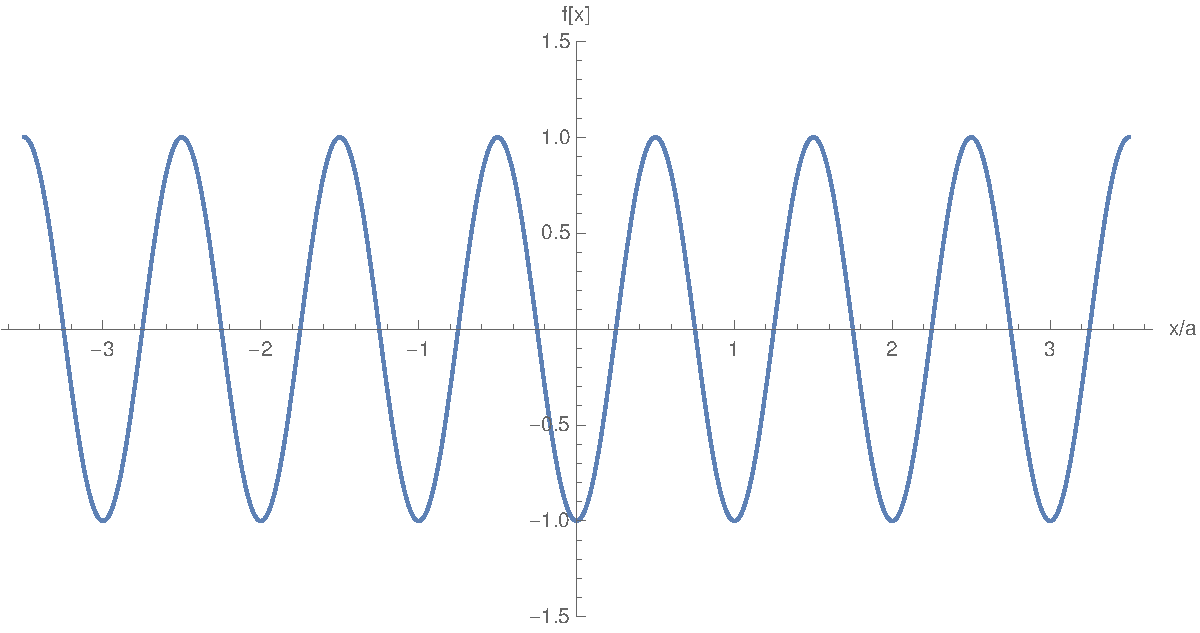
\includegraphics[width=0.3\linewidth]{figures/fPlot}
% \label{fig:fPlot}
% 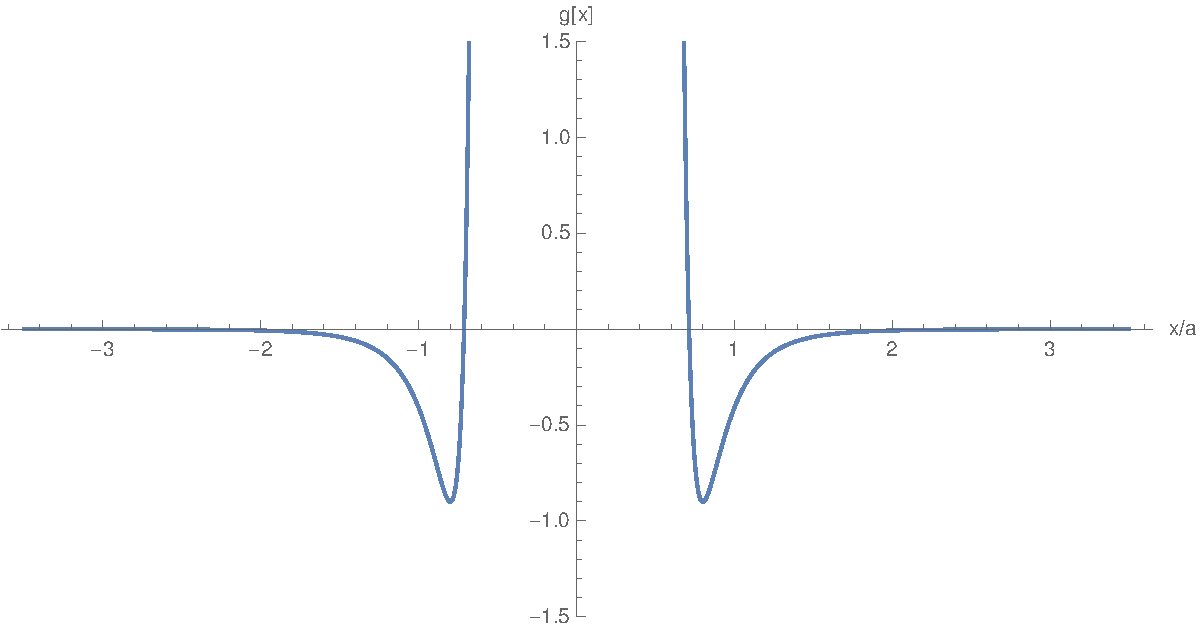
\includegraphics[width=0.3\linewidth]{figures/gPlot}
% \label{fig:gPlot} 
% 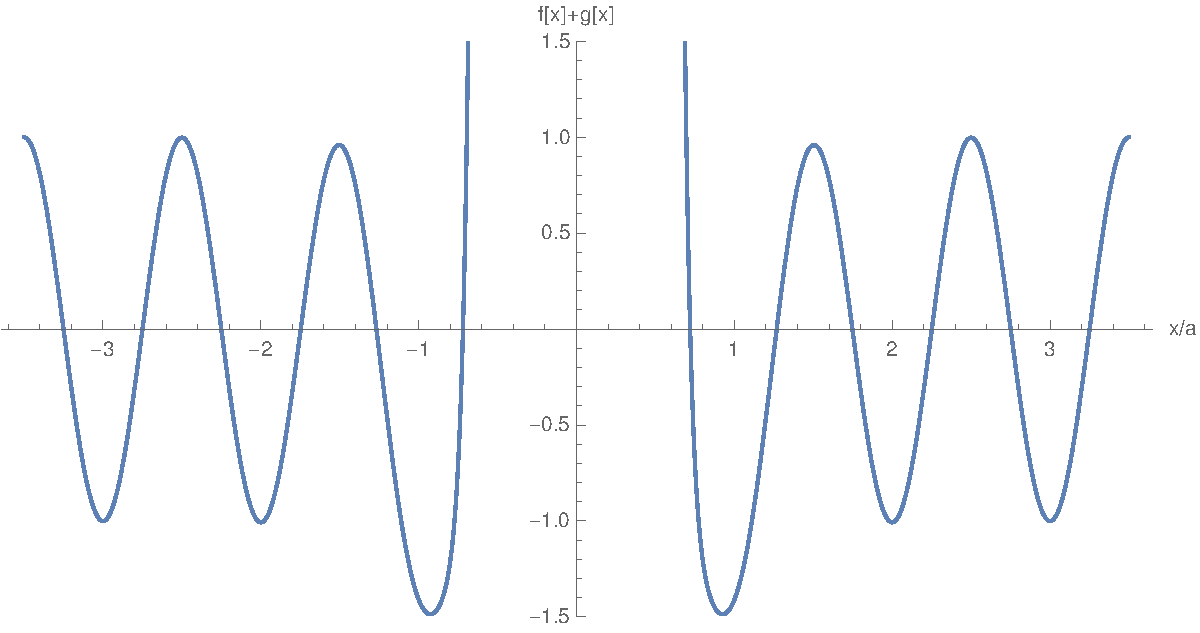
\includegraphics[width=0.3\linewidth]{figures/fgSumPlot}\label{fig:fgSumPlot}
%\end{multicols}
\begin{itemize} \compresslist
 \item Imagine a bunch of identical particles undergoing Brownian motion in a periodic potential with periodicity $a$. Perhaps this potential might look like the one portrayed by $f(x)$ as shown below.
 \item Let's now introduce interactions between these particles, consisting hard-core short range repulsion and slightly longer-ranged attraction, acting over a distance of $\mathcal{O}(a)$.
 Then if we were to place a particle at the origin, the potential felt by another particle would be like $g(x)$.
 \item Therefore the total potential experienced by a particle, the lattice potential plus the particle-particle interaction, would be $f(x)+g(x)$.
\end{itemize}
\vspace{-2.5em}
\begin{center}
\begin{tabular}{c@{\hspace{0.5em}}c@{\hspace{0.5em}}c}
    $f(x)$ & $g(x)$ & $f(x)+g(x)$ \\
    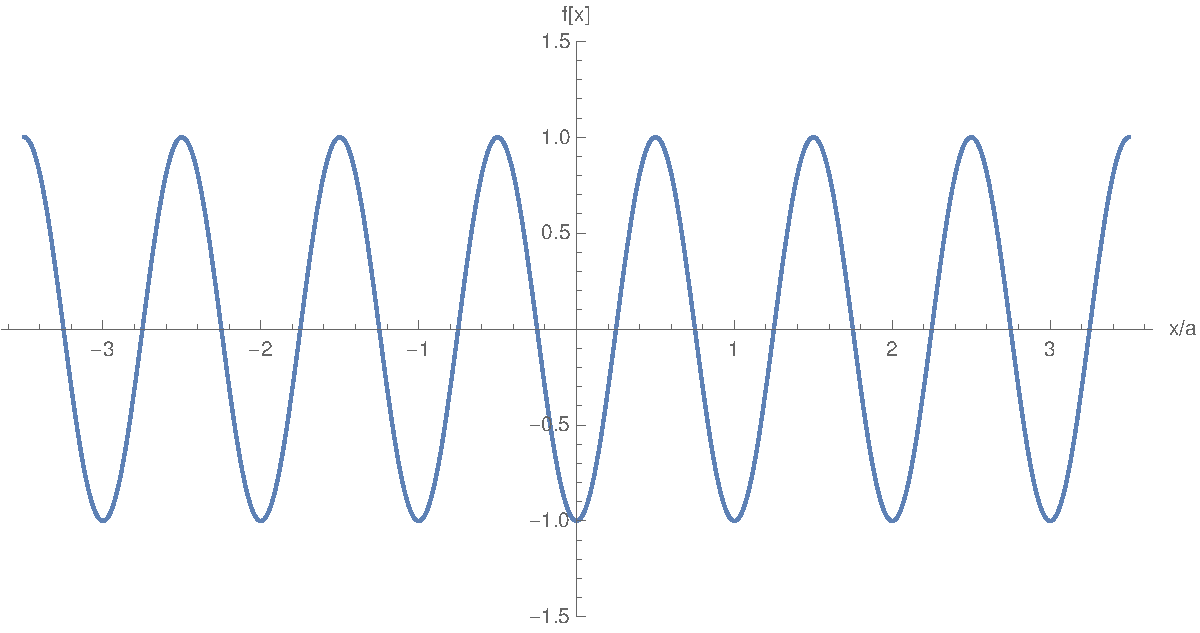
\includegraphics[width=0.32\linewidth]{figures/fPlot} & 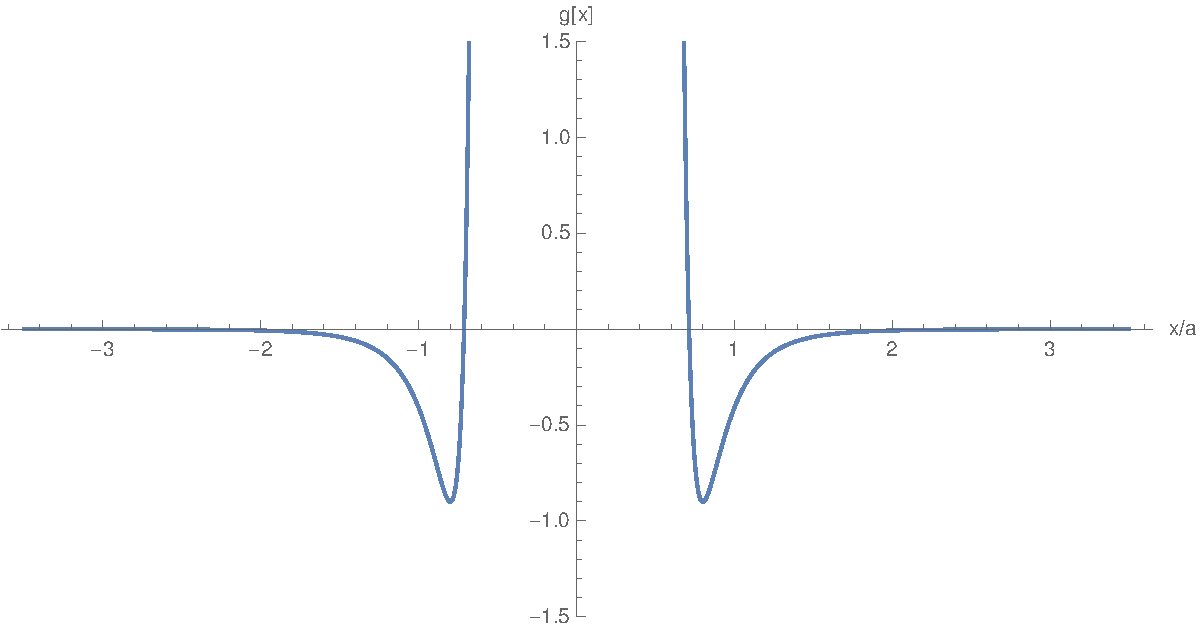
\includegraphics[width=0.32\linewidth]{figures/gPlot} & 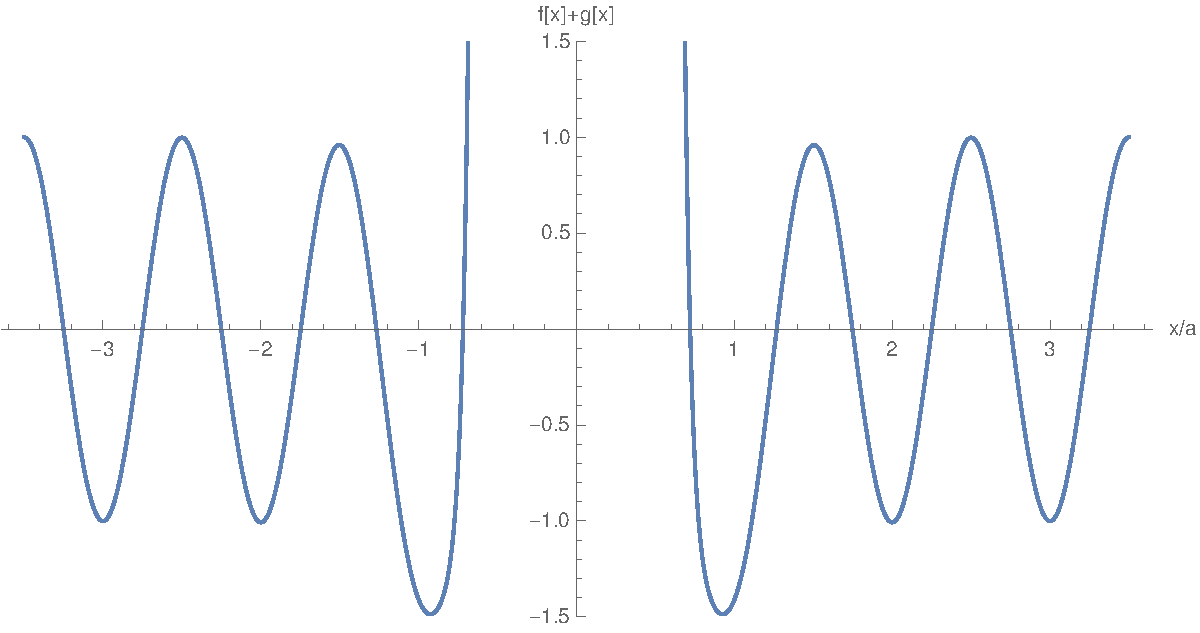
\includegraphics[width=0.32\linewidth]{figures/fgSumPlot} \\
    \end{tabular}
\end{center}
\vspace{-2em}
\begin{itemize} \compresslist
 \item The important thing to note here is that the main difference between the interacting ($f+g$) and noninteracting (only $f$) situations is that a particle wishing to escape the influence
 of an adjacent particle must escape over a taller potential barrier than it usually would. Observe also that only one particle may occupy a potential well at a time, due to the hard-core repulsion.
 \item This motivates us to define a model for particles hopping around on a 1D lattice, defined by the following allowed processes with their associated transition rates:
\end{itemize}
\vspace{-2.5em}
\begin{center}
\begin{tabular}{c@{\hspace{0.5em}}c@{\hspace{0.5em}}c@{\hspace{0.5em}}c}
    
\includegraphics[width=0.24\linewidth]{figures/placeholder} & 
\includegraphics[width=0.24\linewidth]{figures/placeholder} & 
\includegraphics[width=0.24\linewidth]{figures/placeholder} & 
\includegraphics[width=0.24\linewidth]{figures/placeholder} \\
    \end{tabular}
\end{center}
\vspace{-2em}
\begin{itemize} \compresslist
\item More intuitively, particles hop into adjacent empty sites with rate $1$ unless they have a particle already behind them, in which case they hop with rate $\lambda$; the particles are ``sticky'' if $\lambda<1$.
 \item The model I have described sounds pretty generic, and with good reason: this type of ``sticky diffusion'' behaviour happens in numerous situations. I originally made this model in order to investigate the growth of oxide layers
 on the surface of titanium, but it should be quite applicable whenever interacting entities attempt to diffuse through a lattice.
\end{itemize}

%\vspace{0.3em} % When there are two boxes, some whitespace may need to be added if the one on the right has more content
}


%----------------------------------------------------------------------------------------
%	RESULTS
%----------------------------------------------------------------------------------------

\headerbox{Numerical Results}{name=results,column=2,span=2,row=0}{
\begin{itemize}
 \item Our continuum-limit mean-field theory has made some rather wild predictions about backwards diffusion; it would be nice if we had a way to test them.
 \item As luck would have it, the Kinetic Monte Carlo algorithm is ideal for simulating the kind of model we have described. It is implemented via \texttt{Python}-wrapped \texttt{C++}
 in the \texttt{KMCLib} software package\cite{kmclib}.
 \item As of the time of writing, I have not yet confirmed or refuted the MFT current flow predictions. However, I have come across a variety of interesting behaviours exhibited by the model,
 and have included some images of them in the table below.
\end{itemize}
\begin{center}
\begin{tabular}{c p{0.2\linewidth}}
\begin{tabular}{c|c@{\hspace{0.5em}}c@{\hspace{0.5em}}c  }
  &  $\lambda=0.01$ & $\lambda=0.14$ & $\lambda=0.54$ \\ 
  \hline
   $\rho_0=0.11$ & 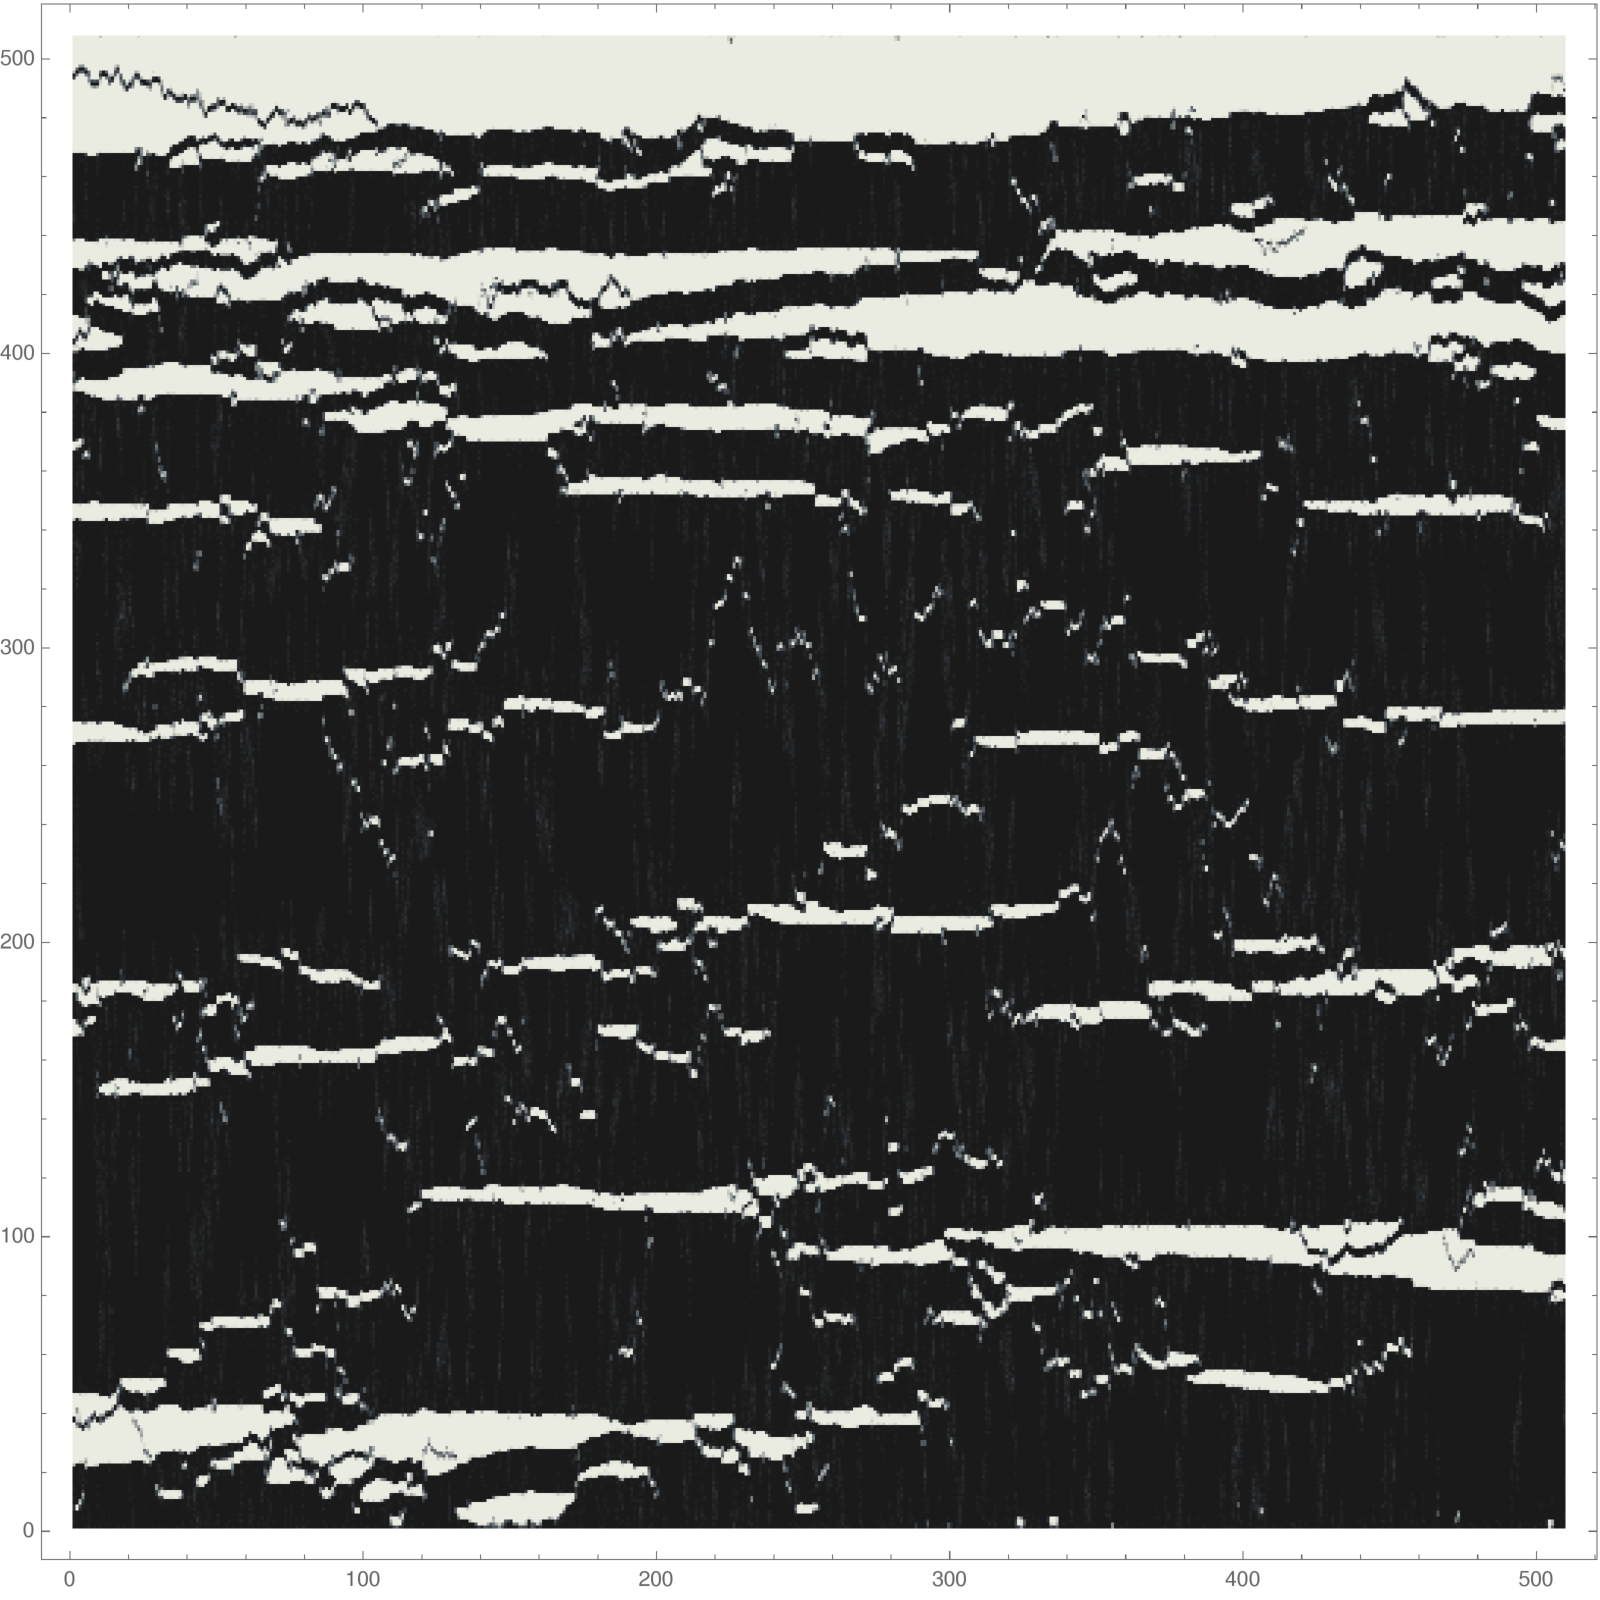
\includegraphics[width=0.2\linewidth]{figures/r_11l_01} & 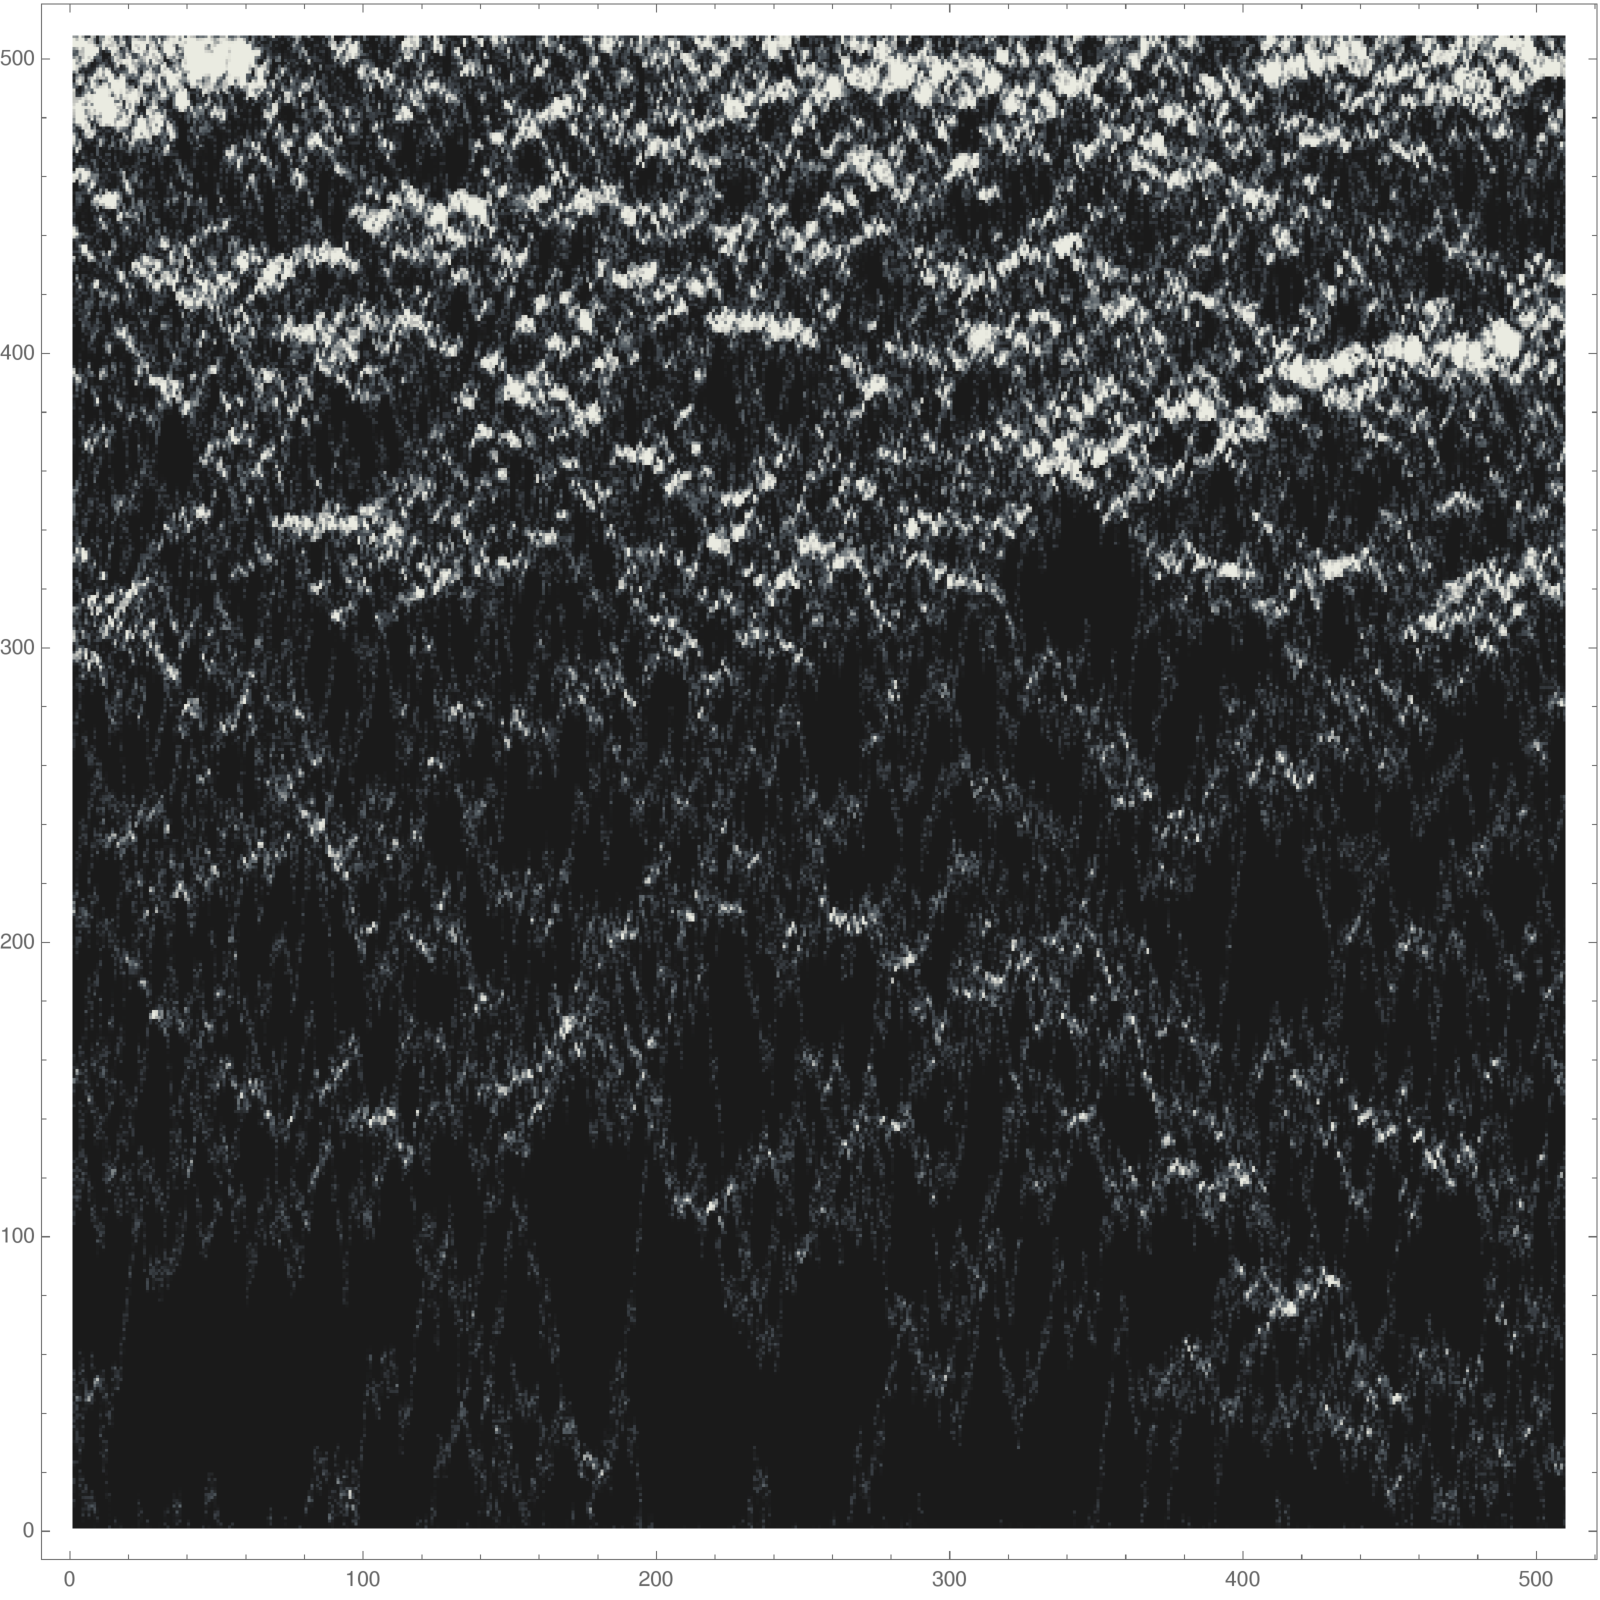
\includegraphics[width=0.2\linewidth]{figures/r_11l_14} & 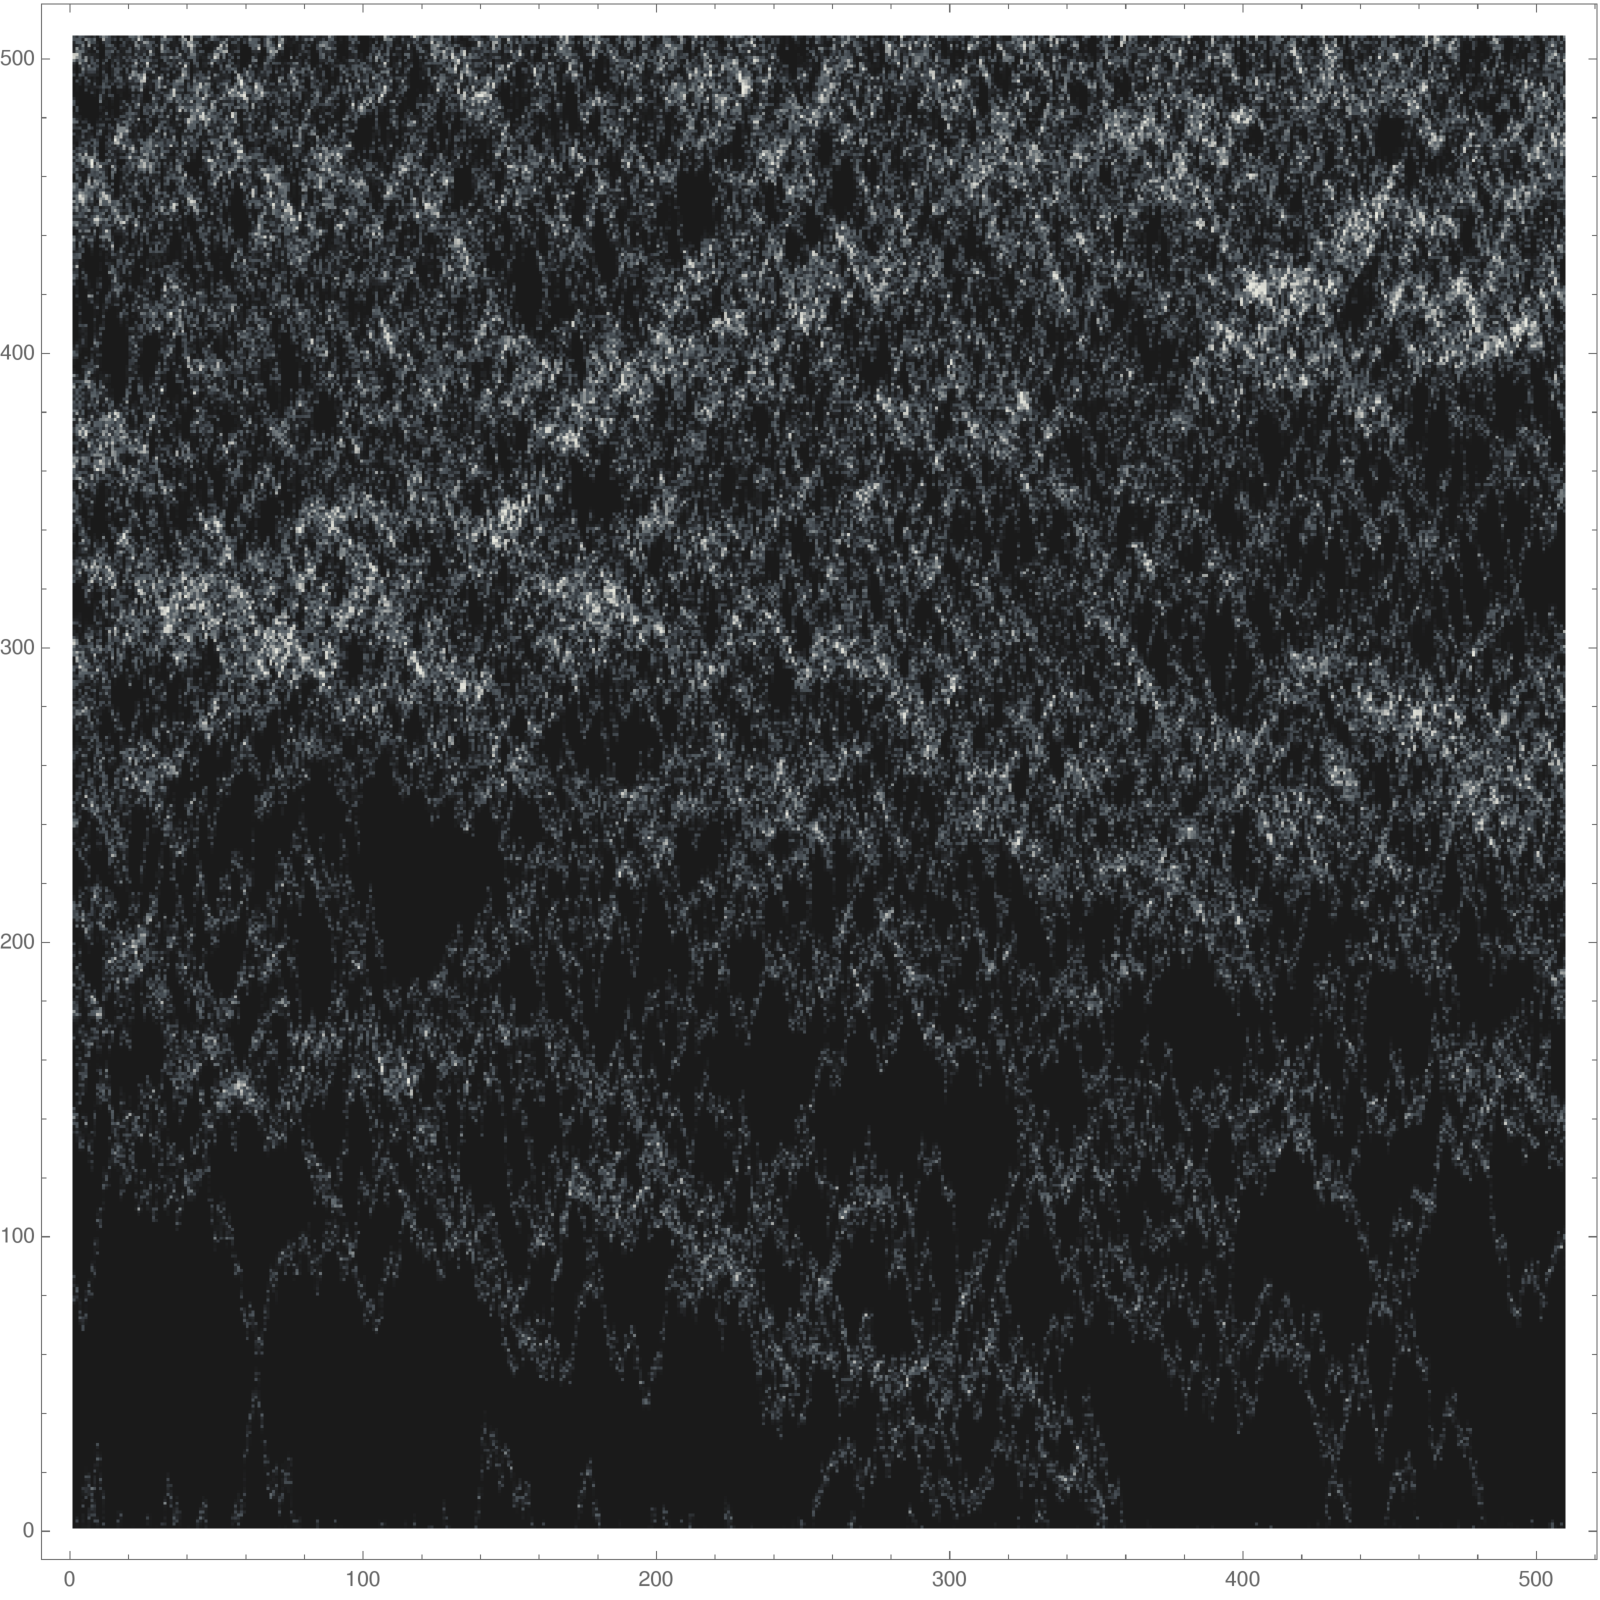
\includegraphics[width=0.2\linewidth]{figures/r_11l_54} \\
   $\rho_0=0.37$ & 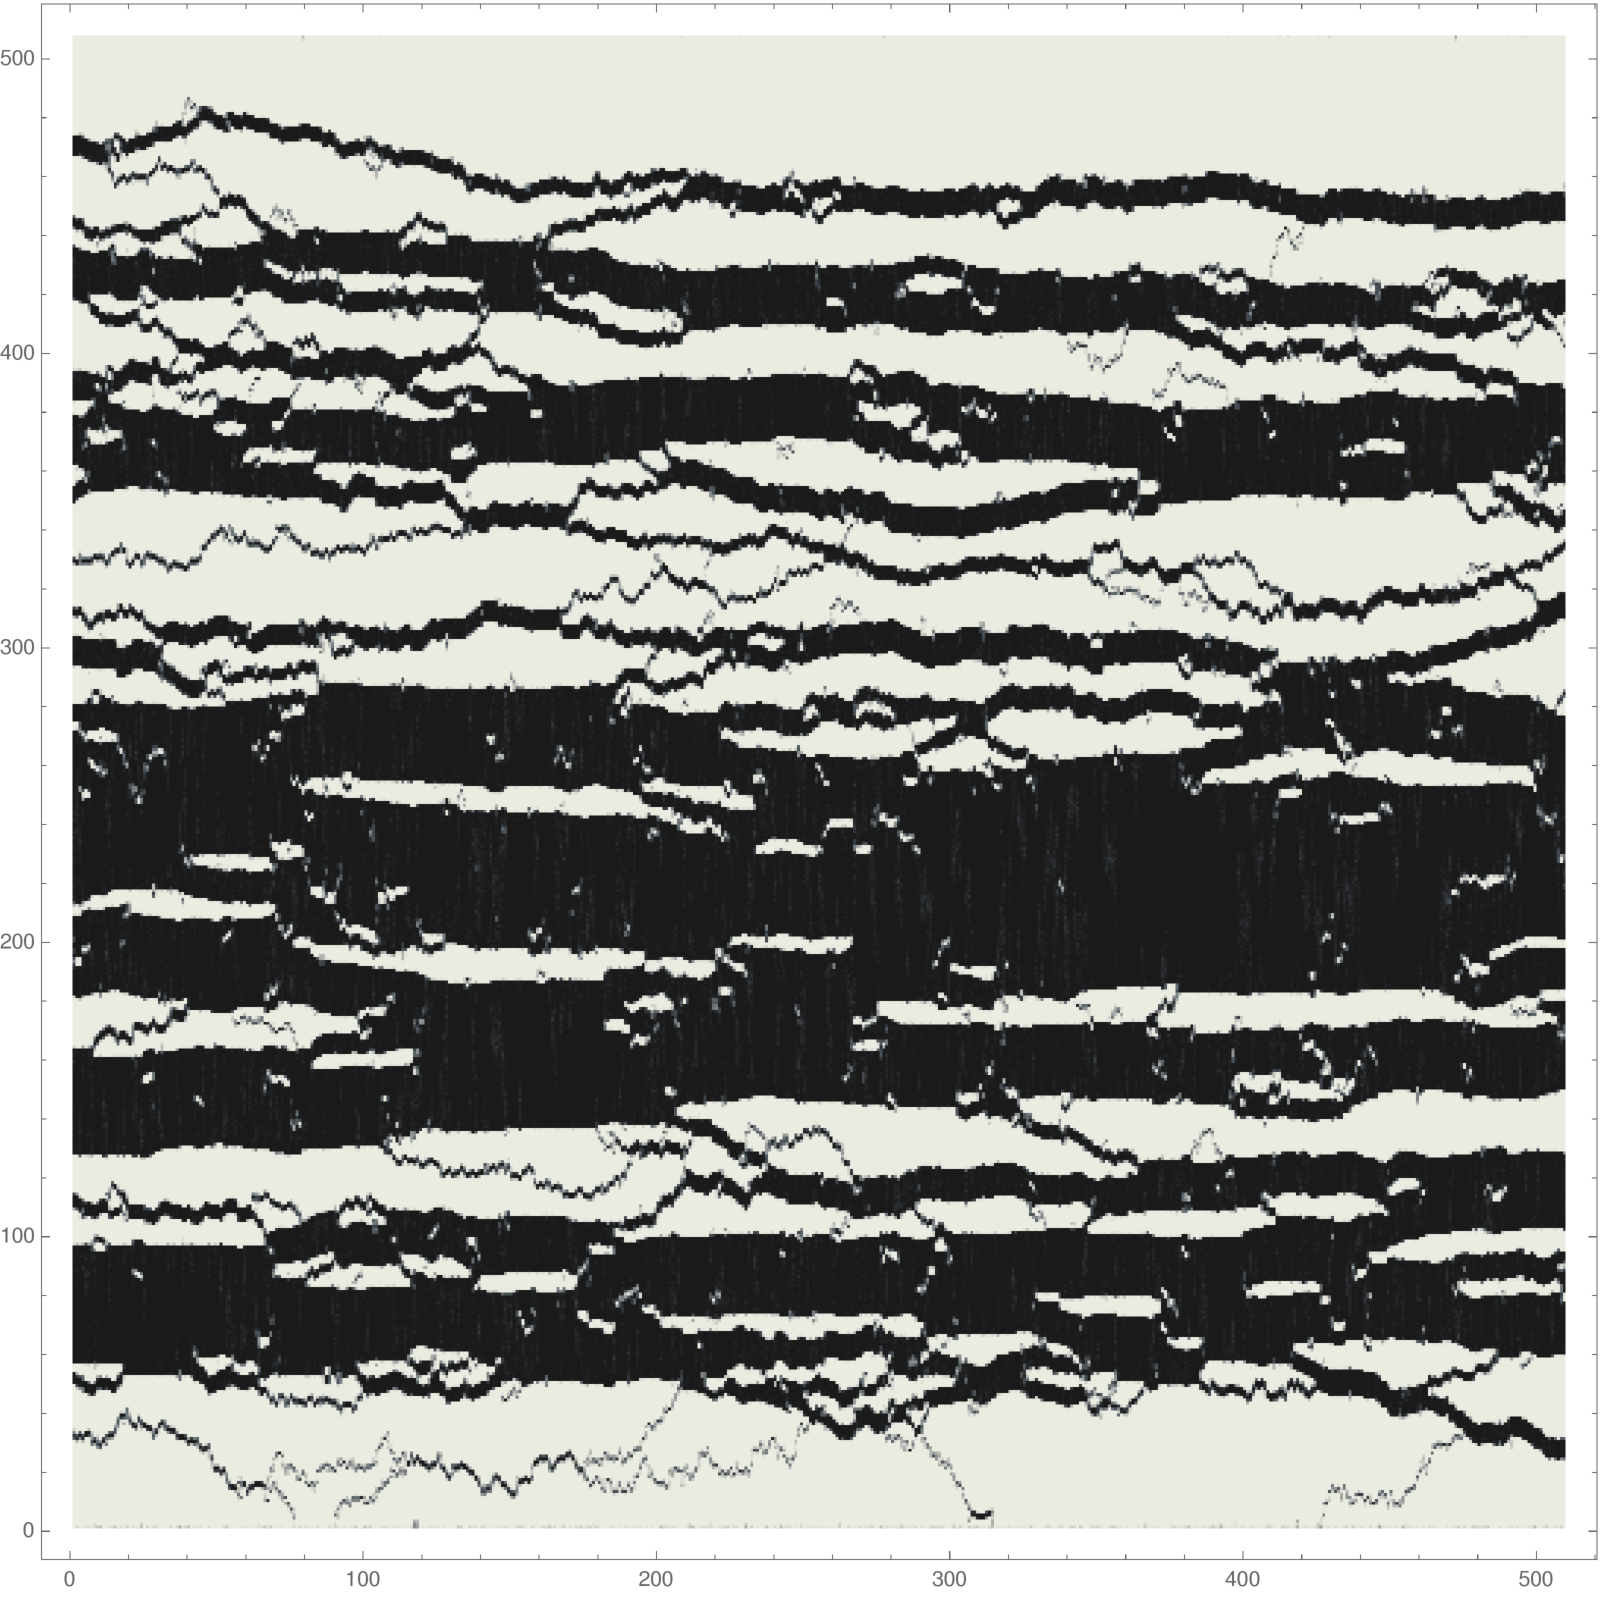
\includegraphics[width=0.2\linewidth]{figures/r_37l_01} & 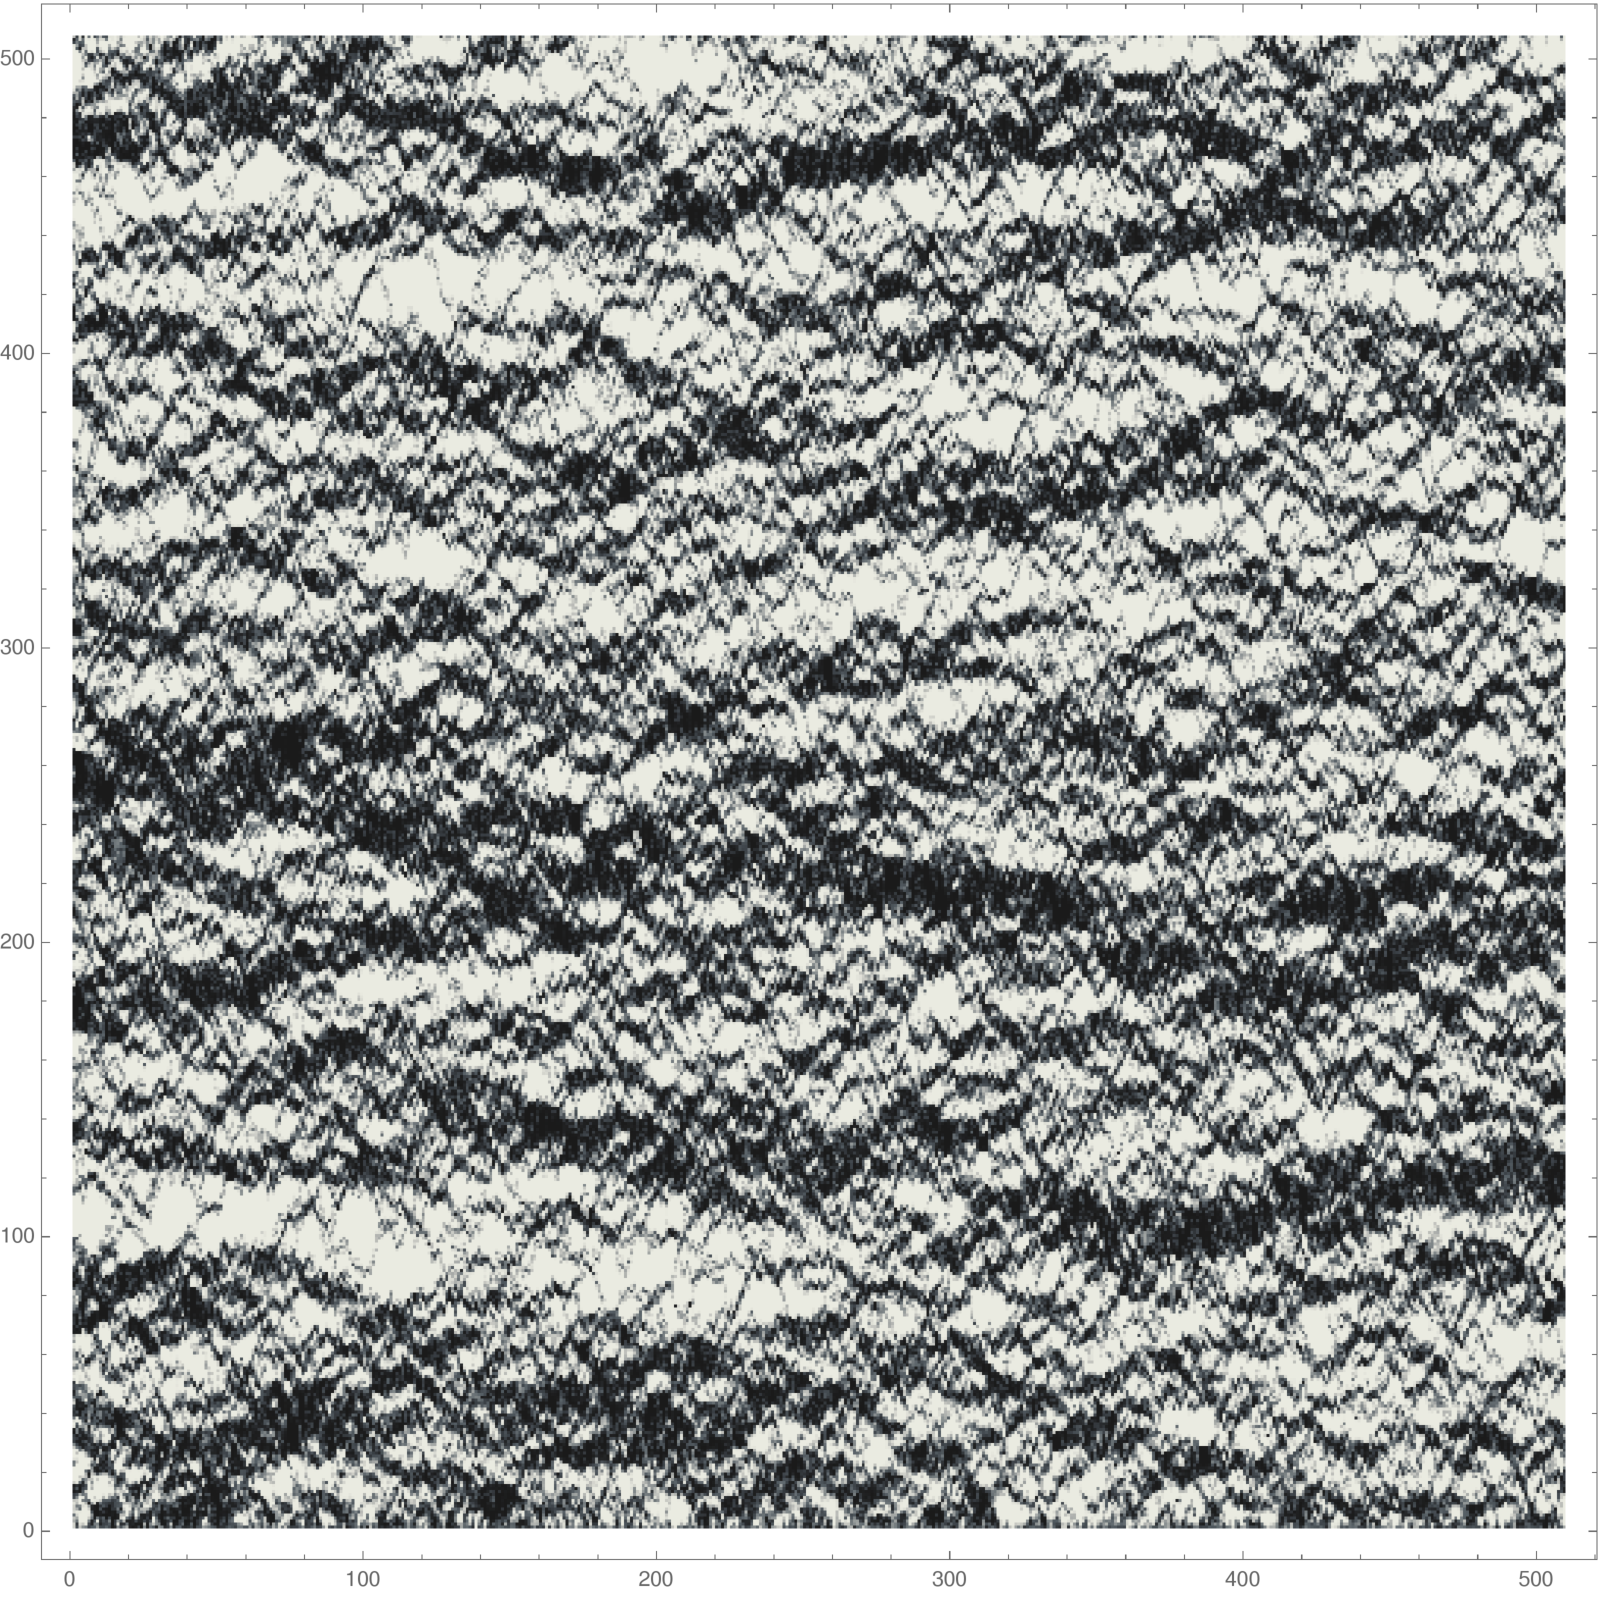
\includegraphics[width=0.2\linewidth]{figures/r_37l_14} & 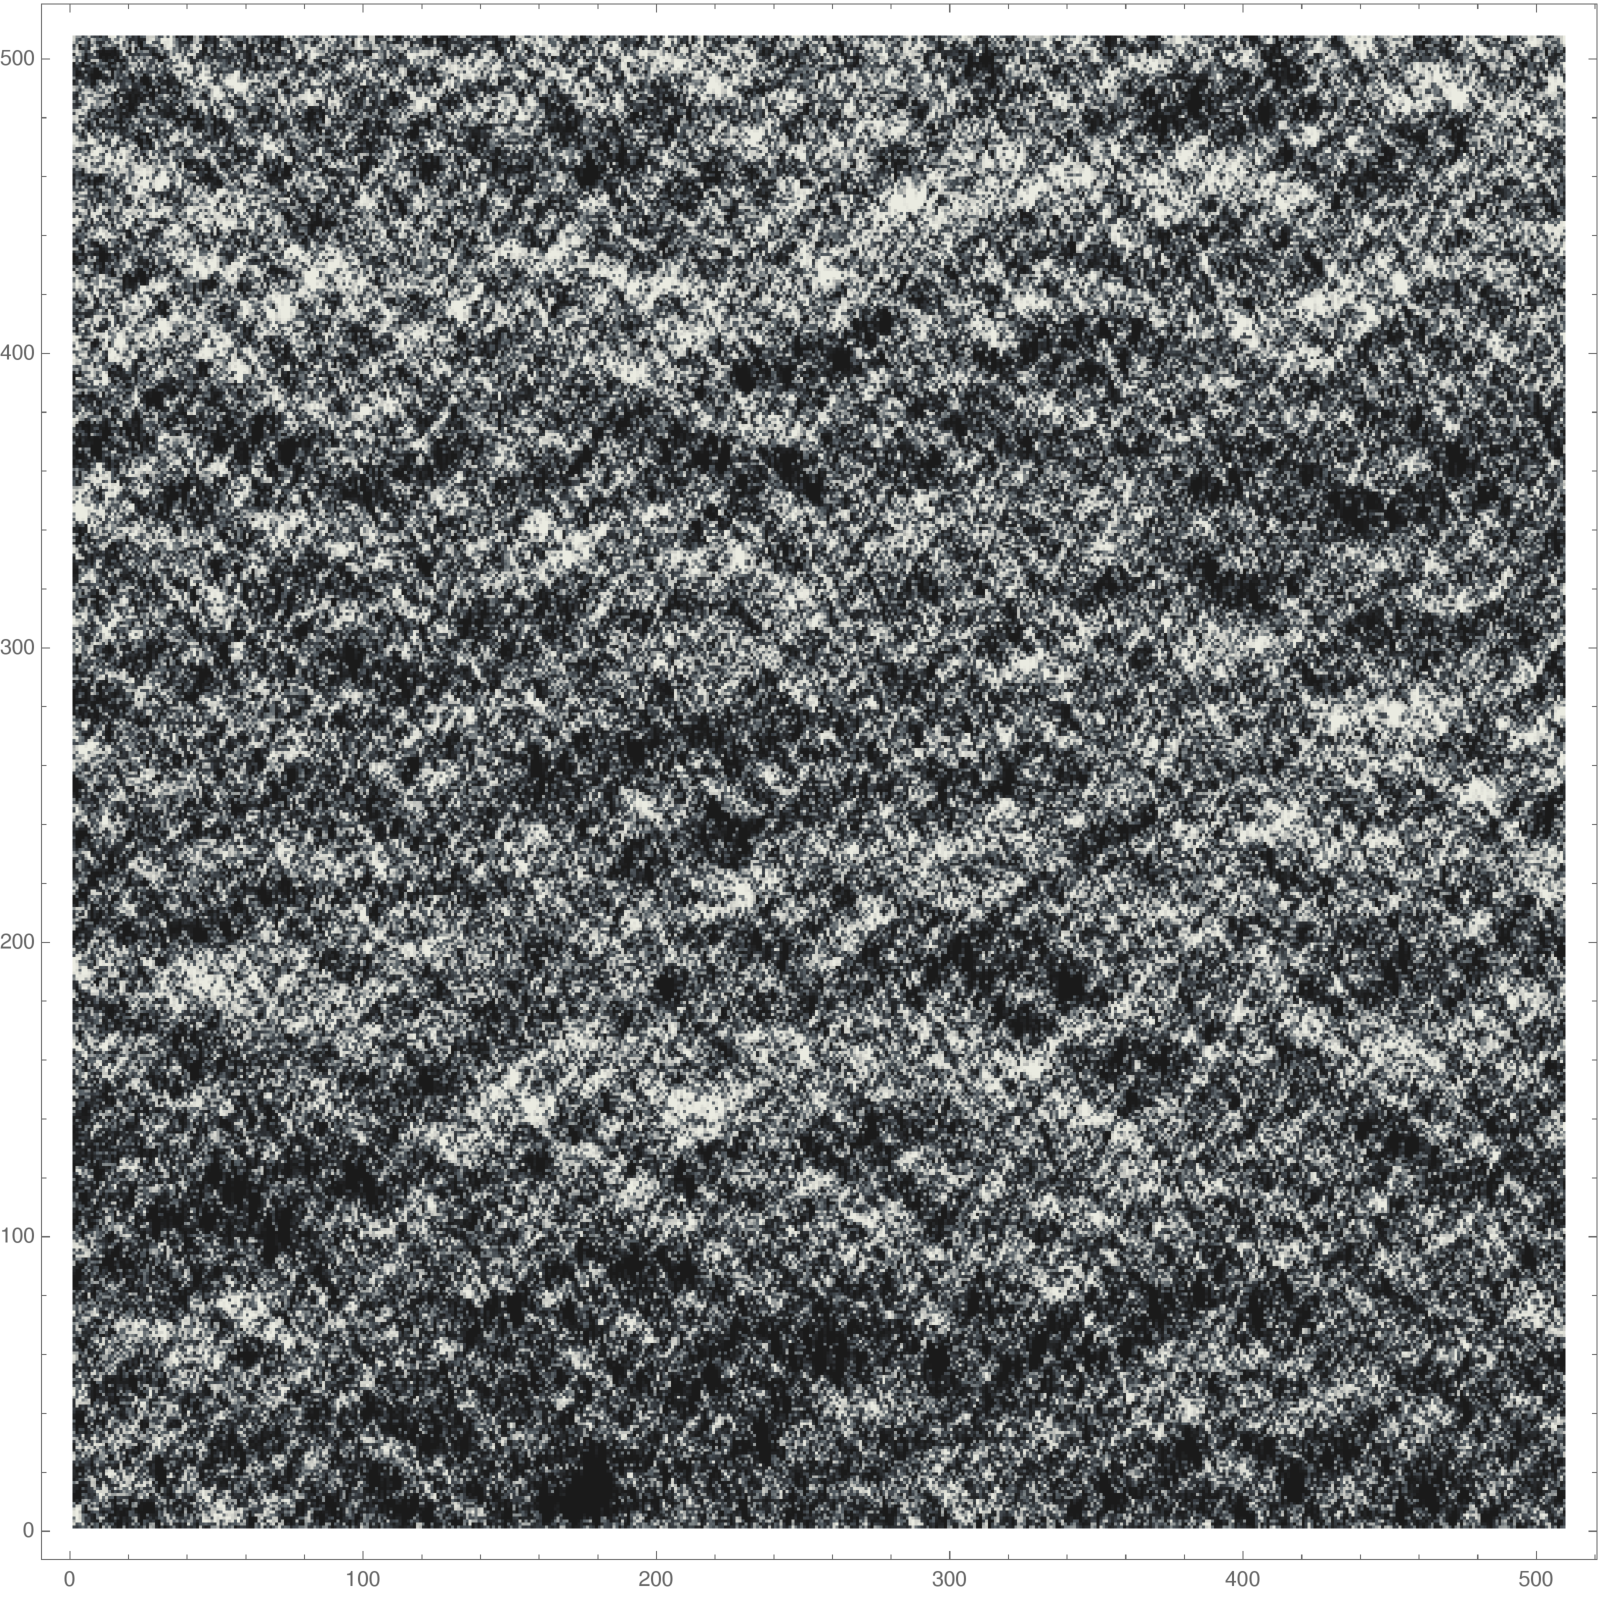
\includegraphics[width=0.2\linewidth]{figures/r_37l_54} \\
   $\rho_0=0.89$ & 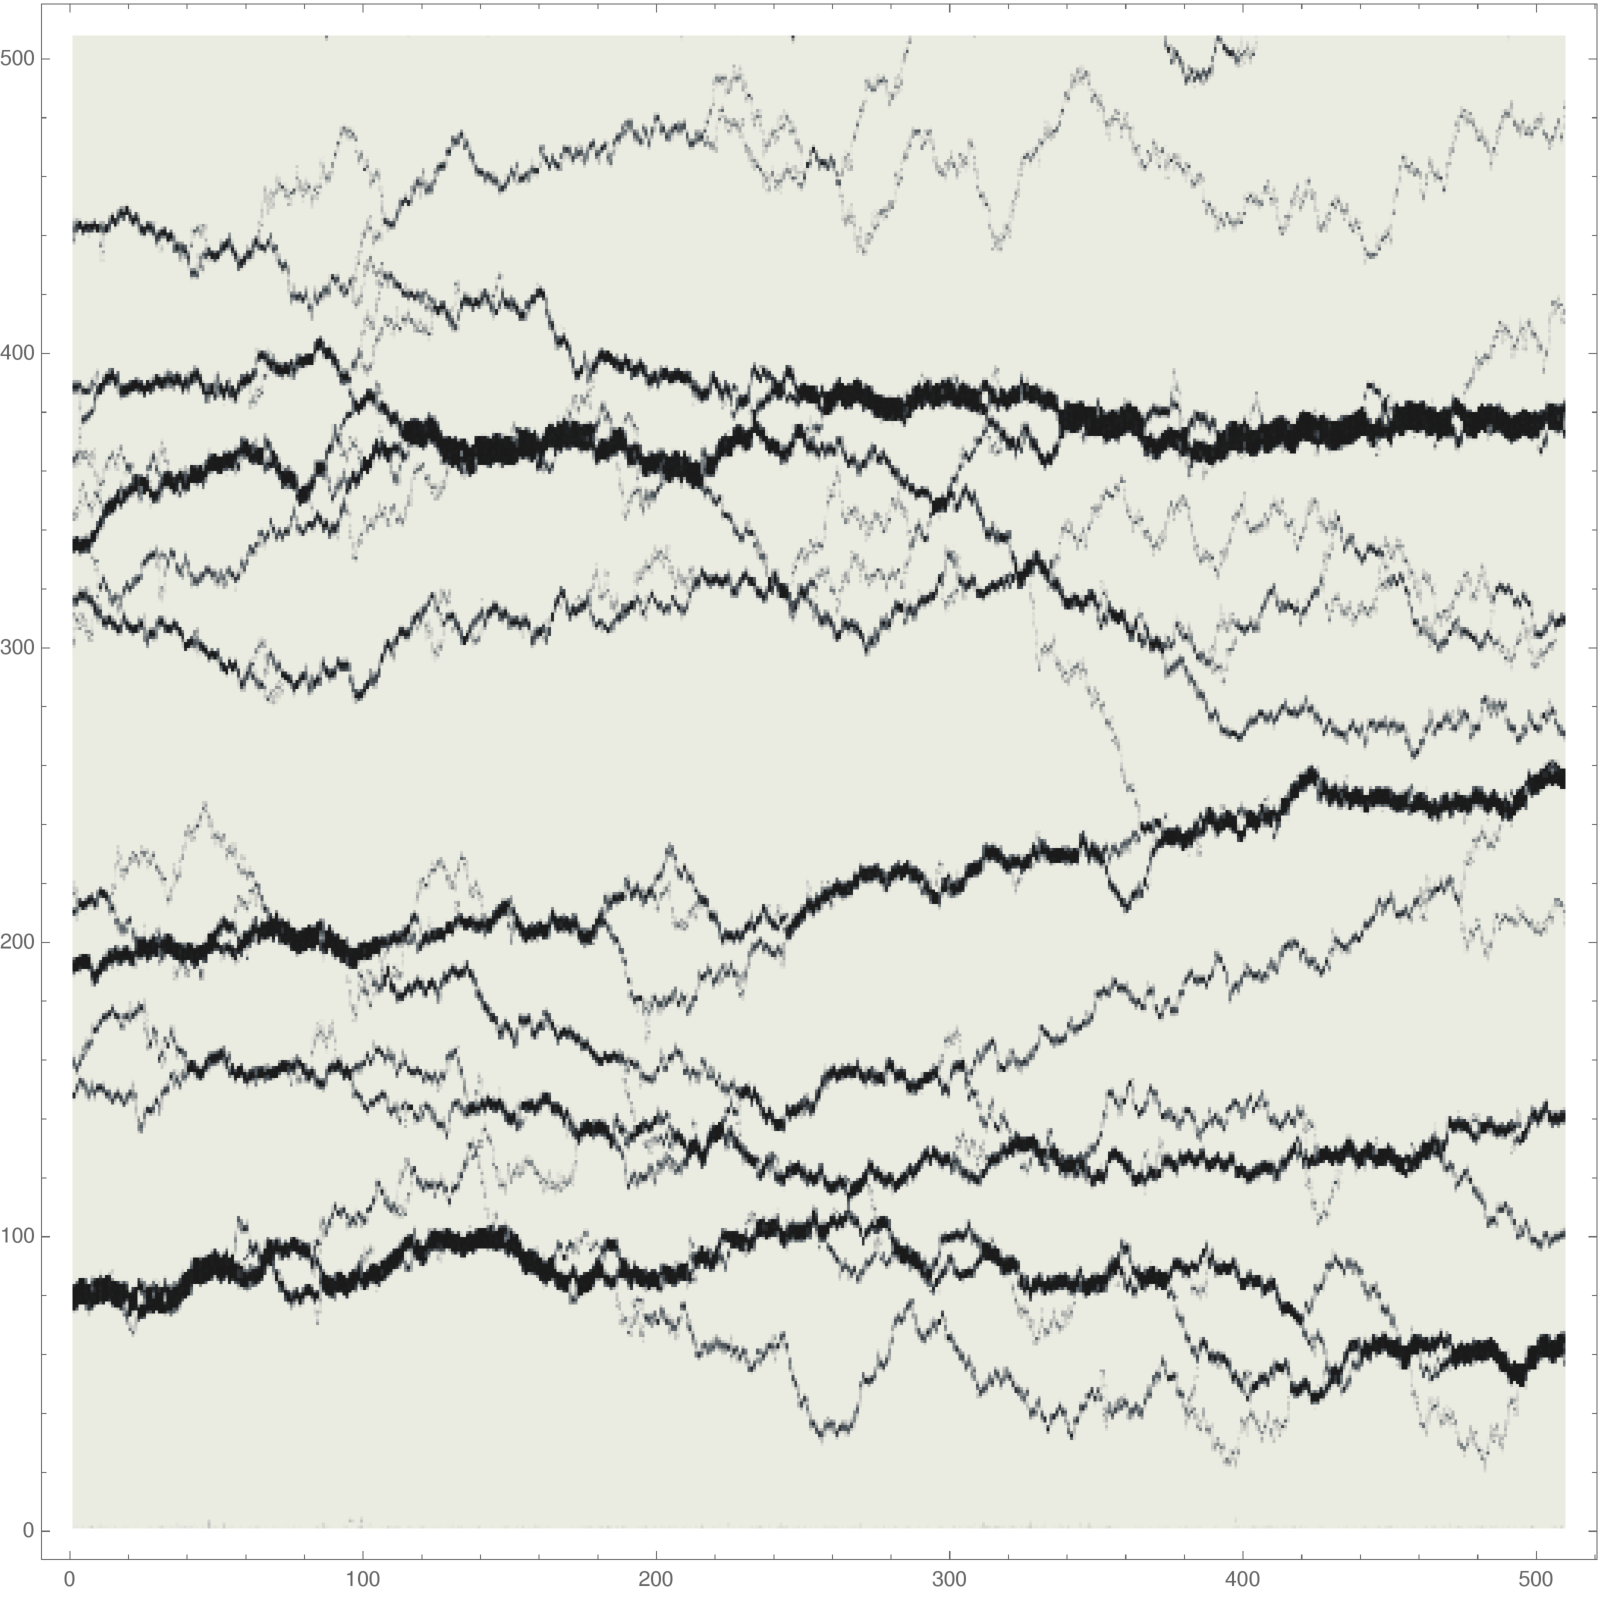
\includegraphics[width=0.2\linewidth]{figures/r_89l_01} & 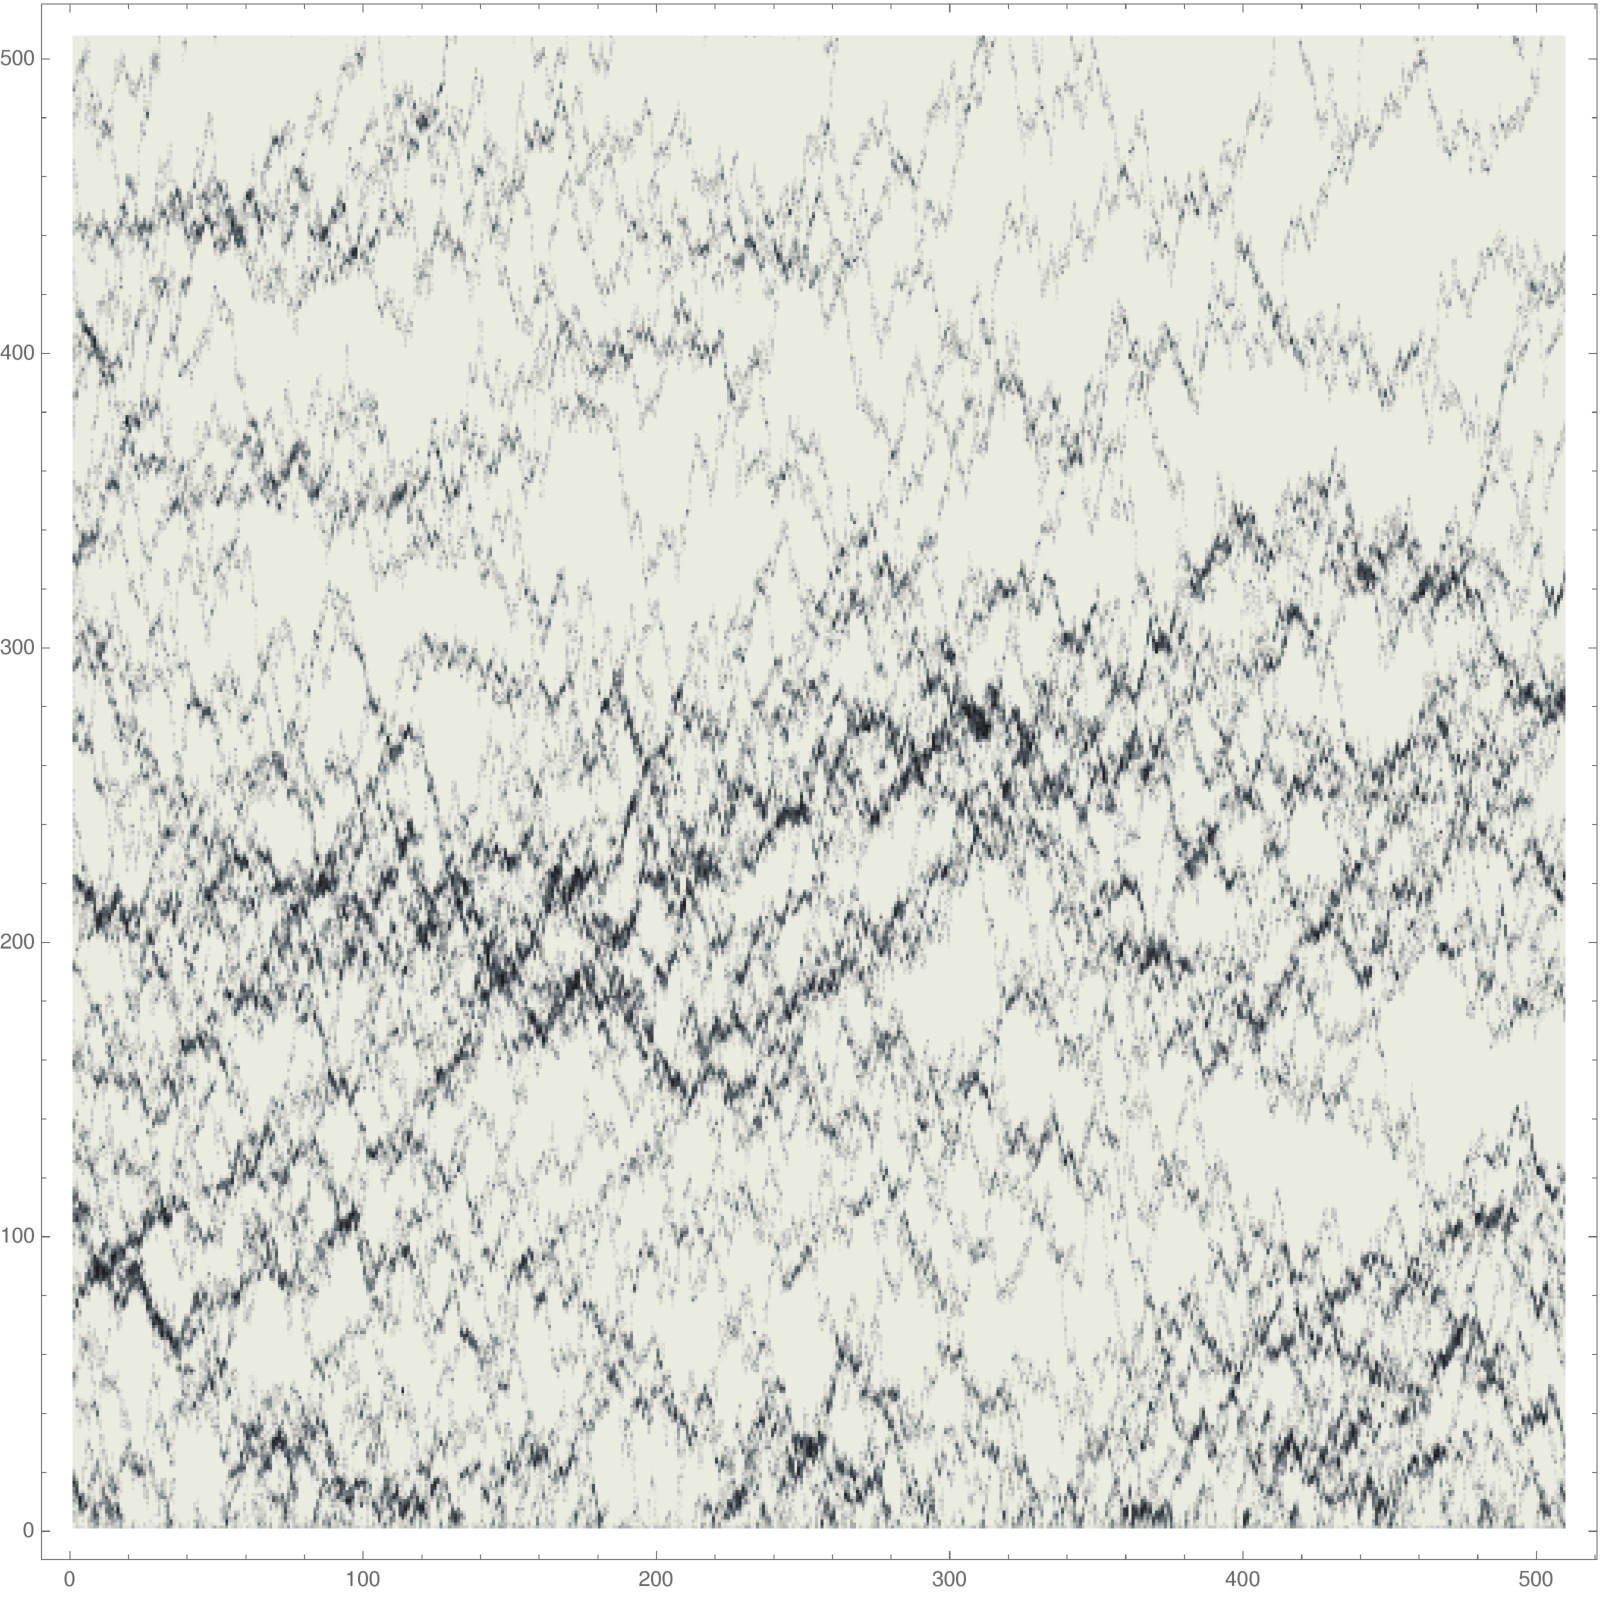
\includegraphics[width=0.2\linewidth]{figures/r_89l_14} & 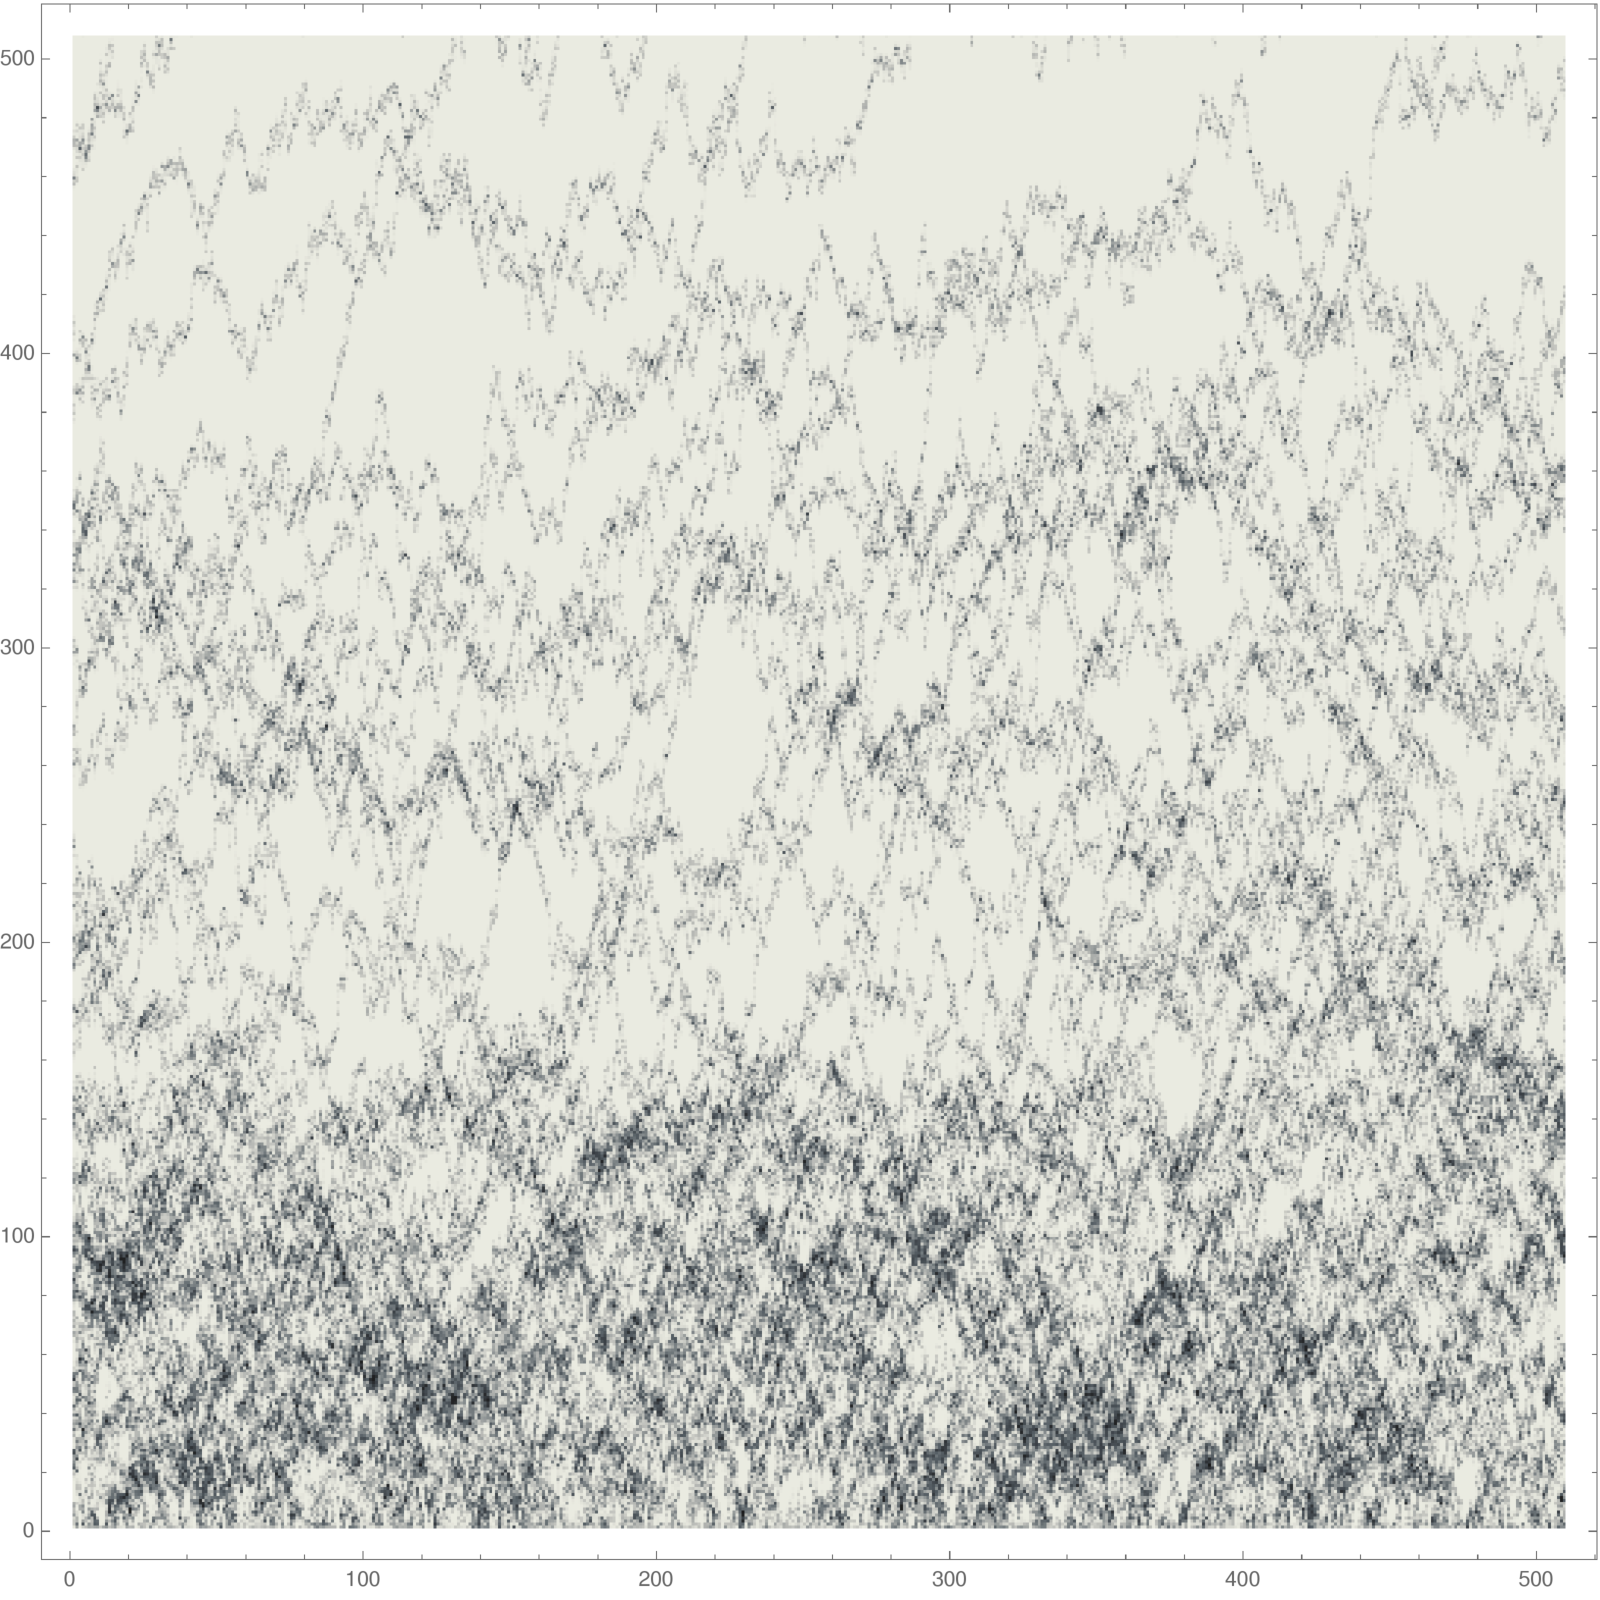
\includegraphics[width=0.2\linewidth]{figures/r_89l_54} \\
\end{tabular}
&
This is where the text would go lol \\
\end{tabular}
\end{center}
%------------------------------------------------
}

%----------------------------------------------------------------------------------------
%	REFERENCES
%----------------------------------------------------------------------------------------

%\headerbox{Acknowledgements and References}{name=ackRef,column=2, span=2, above=bottom}{
%
%\renewcommand{\section}[2]{\vskip 0.05em} % Get rid of the default "References" section title
%\nocite{*} % Insert publications even if they are not cited in the poster
%\small{ % Reduce the font size in this block
%\bibliographystyle{unsrt}
%\bibliography{myBib} % Use myBib.bib as the bibliography file
%}}

%----------------------------------------------------------------------------------------
%	CONCLUSIONS
%----------------------------------------------------------------------------------------

\headerbox{Closing Remarks}{name=closRem,column=2, span=2, below=results, above=bottom}{ % This block is as tall as the references block
Stuff about the future.
\bibliographystyle{unsrt}
\bibliography{myBib} % Use myBib.bib as the bibliography file
}

%----------------------------------------------------------------------------------------
%	PHENO
%----------------------------------------------------------------------------------------

\headerbox{Model Phenomenology}{name=pheno,column=0, span=2, below=intDef, above=bottom}{ % This block's bottom aligns with the bottom of the conclusion block
\begin{itemize} \compresslist
 \item The model described above obeys the detailed balance condition, and after a little relabelling can be shown to be equivalent to the Ising model in equilibrium.
 \item If we move our attention to the large-scale ($a\rightarrow0$) limit and use mean-field theory, we may derive hydrodynamical equations that describe the current, $J$, of the particle density, $\rho$, like a fluid.
 \item In our model, the number of particles is conserved, so we have a continuity equation, $\partial_t \rho + \partial_x J = 0$.
 \item After a little mathematical effort, one may show that $J = -a \left[ 1-(1-\lambda) \left( 4-3\rho \right)\rho \right] \partial_x \rho$ ; current flows down the concentration gradient, in proportion to a coefficient ($\left[ \cdots \right]$)
 which depends upon $\rho$.
 \item When $\lambda<\frac{1}{4}$, it becomes physically possible for that coefficient to be negative; thus, we have a prediction that sometimes particles might flow \textbf{towards} regions of higher concentration!
 \item This runs contrary to our usual intuition about how diffusive systems work\dots
\end{itemize}

}


\end{poster}

\end{document}